\documentclass [a4 paper,11pt]{article}
\usepackage [french]{babel}
\usepackage [utf8]{inputenc}
\usepackage{graphicx}
\usepackage[T1]{fontenc}
\usepackage{textcomp}
\usepackage{listingsutf8}
\usepackage{xcolor}
\usepackage{textcomp}
\usepackage{float}
\usepackage{hyperref}
\usepackage{fancyhdr}
\usepackage{caption}
\usepackage{subcaption}
\usepackage{animate}

\title {Compte rendu TP HMIN320}
\author {
\bsc{LE PHILIPPE} Noé\\
}
\date{\today}

\begin{document}
\makeatletter
 
\maketitle
\section{Compte rendu TP1}
\subsection{Disclaimer}
Il serait malhonnête de prétendre avoir compris quoi que ce soit au TP, mon niveau en mathématiques n'est clairement pas suffisant. Fort heureusement pour moi, je suis meilleur développeur que mathématicien, et j'ai tout de même réussi à m'en sortir. Je présenterai donc mes résultats dans ce rapport, et ce que j'ai pu comprendre et extraire comme connaissances.


\subsection{Calcul de la matrice fondamentale}
La précision de la sélection des paires de points (fig. \ref{fig:pts1}, fig. \ref{fig:pts2}) semble importante dans le calcul de la matrice fondamentale, mais même avec une matrice fondamentale différente, les résultats, comme nous le verrons, bien que différents, semblent tous être corrects.

\begin{figure}
\centering
\begin{subfigure}{0.5\textwidth}
  \centering
  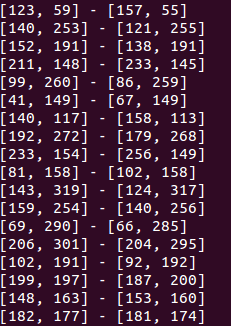
\includegraphics[width=0.8\linewidth]{pts1.png}
  \caption{Première série de points}
  \label{fig:pts1}
\end{subfigure}%
\begin{subfigure}{0.5\textwidth}
  \centering
  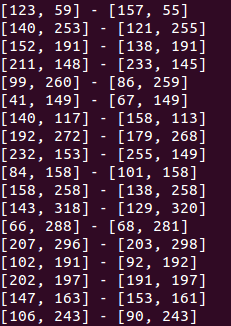
\includegraphics[width=0.8\linewidth]{pts2.png}
  \caption{Deuxième série de points}
  \label{fig:pts2}
\end{subfigure}
\caption{Points sélectionnés pour calculer la matrice fondamentale}
\label{fig:pts}
\end{figure}

\begin{figure}
  \centering
  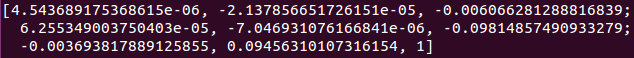
\includegraphics[width=0.8\linewidth]{mat1.png}
  \caption{Matrice de la première série de points}
  \label{fig:mat1}
\end{figure}%

\begin{figure}
  \centering
  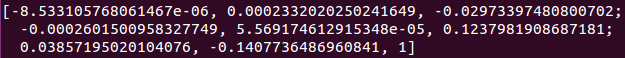
\includegraphics[width=0.8\linewidth]{mat2.png}
  \caption{Matrice de la deuxième série de points}
  \label{fig:mat2}
\end{figure}%

Les matrices fondamentales (fig. \ref{fig:mat1}, fig. \ref{fig:mat2}) ont des têtes de matrices fondamentales, mais difficile de dire plus, ou de les valider, si ce n'est experimentalement.

\newpage

\subsection{Validation de la matrice}
Pour vérifier que la matrice fondamentale est correcte et cohérente, j'ai tracé les droites épipolaires des points de controle (fig. \ref{fig:epipole1}, fig. \ref{fig:epipole2}). Si toutes les droites s'intersectent en un même point (l'épipole) en passant par leur point de controle respectif, c'est que la matrice fondamentale est correcte. On voit que l'épipole est très différent, les droites semblent cependant bien converger et passer, à quelques erreurs près, par les points de controle.

\begin{figure}
  \centering
  \begin{subfigure}{0.5\textwidth}
    \centering
    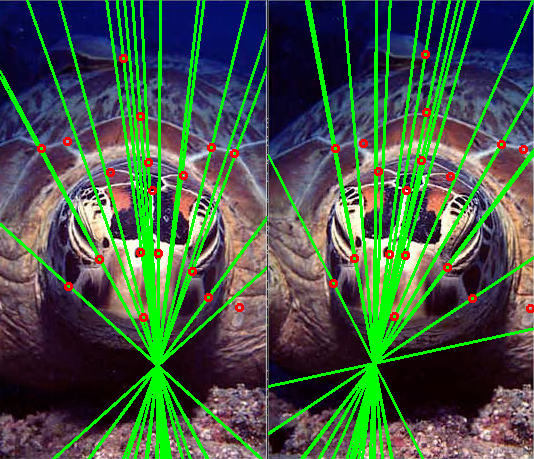
\includegraphics[width=0.8\linewidth]{epipole1.png}
    \caption{Premier épipole}
    \label{fig:epipole1}
  \end{subfigure}%
  \begin{subfigure}{0.5\textwidth}
    \centering
    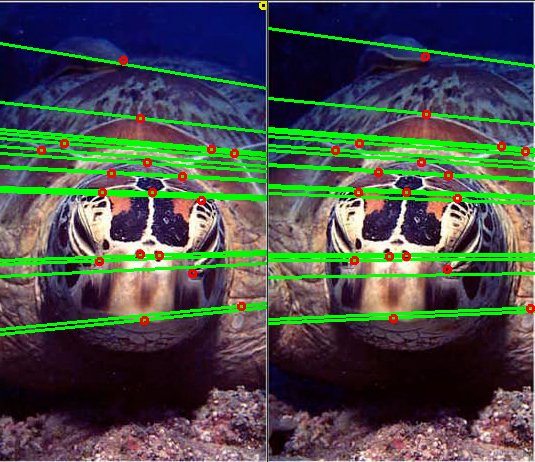
\includegraphics[width=0.8\linewidth]{epipole2.png}
    \caption{Deuxième épipole}
    \label{fig:epipole2}
  \end{subfigure}
  \caption{Épipoles différents avec des matrices différentes}
  \label{fig:epipole}
\end{figure}

\subsection{Droites épipolaires}

Maintenant qu'on sait que la matrice fondamentale calculée est correcte, on peut afficher les droites épipolaires. On peut voir (fig. \ref{fig:droite}) que la précision est relativement bonne, même si certaines droites ne passent pas exactement là où elles doivent passer.

\begin{figure}
  \centering
  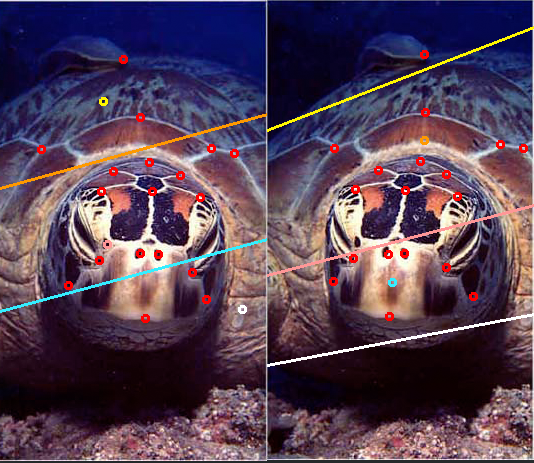
\includegraphics[width=0.8\linewidth]{ptsepipole.png}
  \caption{Droites épipolaires, le point d'une certaine couleur sur une image correspond à la droite épipolaire de la même couleur sur l'autre image. Les points de controle sont en rouge}
  \label{fig:droite}
\end{figure}%

\newpage
\section{TP2}
\subsection{Flot optique}
La fig. \ref{fig:ghost} montre le tracking avec un flot optique. Si le gif ne marche pas, j'ai joint les images dans une archive dans le mail.
\newpage
\begin{figure}
\centering
\animategraphics[controls,autoplay,loop,scale=0.5]{12}{TP2/out/out}{0}{18}
\caption{Tracking sur les images}
\label{fig:ghost}
\end{figure}
\end{document}

